\documentclass[12pt,oneside,letterpaper]{article}

\usepackage{graphicx}
\usepackage[font=small,labelfont=bf]{caption}
\pagestyle{headings}
\oddsidemargin 0.25in \textwidth     6.25in \topmargin     0.4in
\textheight    8.5in

\begin{document}


\title{\bfseries Data Classifier: \\
Software Architecture\\
Version 1.0}

\author {
\large{Team Mark}\\
\emph{Computer Science Department}\\
\emph{California Polytechnic State University}\\
\emph{San Luis Obispo, CA USA}\\
}

\date{November 7, 2018}
\maketitle \thispagestyle{empty}

\pagebreak
\tableofcontents

\addcontentsline{toc}{section}{Revision History}

\addcontentsline{toc}{section}{Credits}

\section*{Credits}
\begin{tabular}{|l|l|p{2.5in}|l|}
\hline
\textbf{Name}&\textbf{Date}&\textbf{Role}&\textbf{Version}\\
\hline
Matt Yamolich &November 7, 2018&Contributing Member&1.0\\
\hline
Spencer Schurk&November 7, 2018&Lead Author of Introduction&1.0\\
\hline
Sally Jones&October 10, 2009&Lead Author of Business Requirements&1.0\\
\hline
&&&\\
\hline
&&&\\
\hline
\end{tabular}

\section*{Revision History}
\begin{tabular}{|l|l|p{2.5in}|l|}
\hline
\textbf{Name}&\textbf{Date}&\textbf{Reason for Changes}&\textbf{Version}\\
\hline
Spencer Schurk&November 7, 2018&Completed Introduction&1.0\\
\hline
&&&\\
\hline
&&&\\
\hline
&&&\\
\hline
\end{tabular}

\newpage

\section{Introduction}

The purpose of this document is to describe the architecture of our Data Classifier. This document will be used as a reference when development begins. This document may change over time as we learn more about specific technologies being used for this project. For more information regarding this project, please see the Vision and Scope document, as well as the SRS document.

\section{Problem Description}
[Tell the audience what problem is being solved, or requirements are being met, by this design.  Include requirements or constraints that drive the direction of the design.

Any quality attribute requirements or constraints should also be explained in this section.]



\section{Solution}
This project is meant as an interface between a database and the data being inputted to it by the user. The main goal of this project is to provide analytics for the user in order to better identify what type of data is being inputted. With this project, the user will be able to tell the categories of data being inputted, and how they potentially relate to each other. The classifier will allow the user to modify these relations and to interact with a visual model based on these interactions. As defined by the customer, the user will interact with a web based GUI, most likely based on React. This GUI will interface with the Python backend, which is another design restraint, and utilize Scikit, a python library, as our chosen machine classifier. This classifier will act as the main interface/buffer between the user and actually logging the data to the database. 

\subsection{Overview}
[This section should be a summary of the solution in a few paragraphs, preferably less than a page.]

\subsection{Components}
[This section should list and briefly describe the components of the design.  The word ``components'' can refer to deployable units or to areas of the design, as appropriate. This section should start with the deployment diagram.]

\subsection{Design}
[This is where the meat of the design lives.  For each component, there should be a subsection describing the design of that component in as much detail as you want to provide in a high-level design.  There should also be a subsection that describes how the components work together. This section should include class, sequence, and collaboration diagrams as appropriate.]

\subsubsection{Classification Structure}
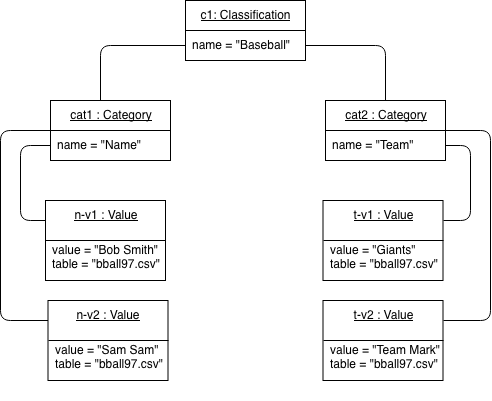
\includegraphics[scale = 0.9]{spencer_object.png}
\begingroup
\captionof{figure}{Data Classification Object Diagram - Spencer Schurk}
\endgroup

\paragraph{} Figure 1 depicts the architecture of our Classification object. Once data classification has completed on the provided files, the finalized result will be structured like this. A classification consists of one Classification object, which contains a String called name, and one to many Categories. 
\paragraph{} Categories are what the classified data is sorted into by the machine learning algorithms. A category consists of a String called name, and one to many values.
\paragraph{} Values are the object representation of one value in a data set. The Value object contains the value, and a reference to the table in which it came from. More attributes may be stored in the Value object as necessary.

\subsubsection{Uploading Files}
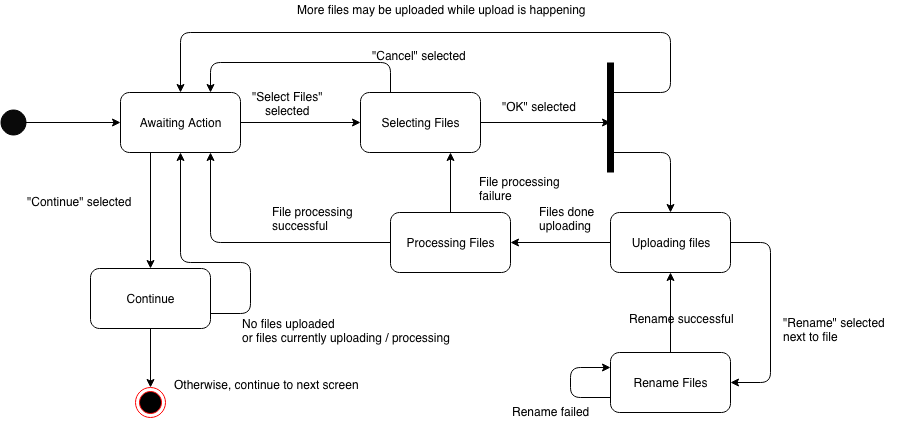
\includegraphics[scale = 0.52]{spencer_state.png}
\begingroup
\captionof{figure}{Upload Files State Diagram - Spencer Schurk}
\endgroup


\paragraph{}Figure 3 models the sequence of the data through the system, and the interaction between the user and the system. Users will begin their interaction with the UI by uploading files to the front-end. Then it will be processed into a temporary holding database for processing, fed to the machine learning algorithm, then the resulting data will be displayed by the UI.
\paragraph{} Since this process can happen multiple times, there must be a cleanup for purging the temporary database so that unwanted/sensitive data is not stored permanently in an potentially unsecured/unknown entry.
\paragraph{} This process will then repeat per data entry uploaded by the user and can be repeated as many times as the user desires.

\subsubsection{Overview of Classes}
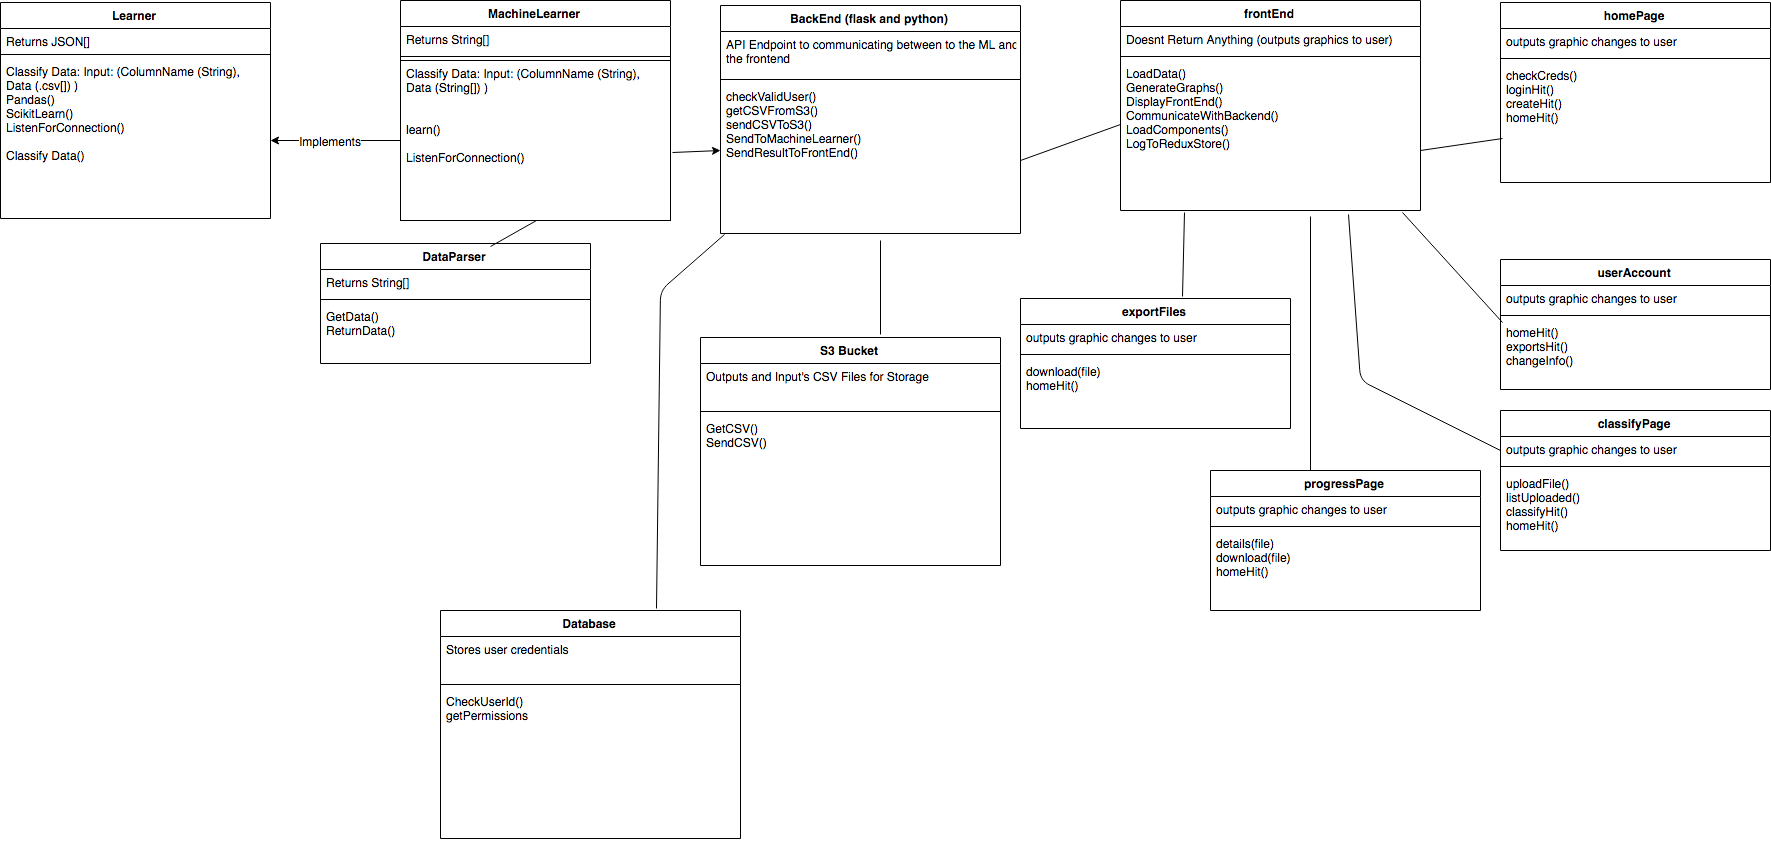
\includegraphics[scale = 0.3]{YarmClassDiagram.png}
\begingroup
\captionof{figure}{Overview of Classes - Matt Yarmolich}
\endgroup

\paragraph{} Figure 2 depicts a state diagram modeling the user flow when uploading files to be classified. Users will enter this page from the main menu, and leaving this page will take users to the start of the classification process. When leaving this state, all files that were in the process of being uploaded must be completed or canceled.
\paragraph{} Since users may select more files to upload while some files are already in the process of uploading, a fork is used in this diagram. This means that while files are uploading, a user may select more files to upload, then begin uploading those files. Selecting "continue" will not continue to the next page unless all files have completely uploaded or have been canceled.
\paragraph{} The processing files state may fail for numerous reasons, such as an incompatible file type, or a corrupt file. When this occurs, that file is deleted from the system, and users may select another file to upload, or cancel.

\subsubsection{Flow of Data}
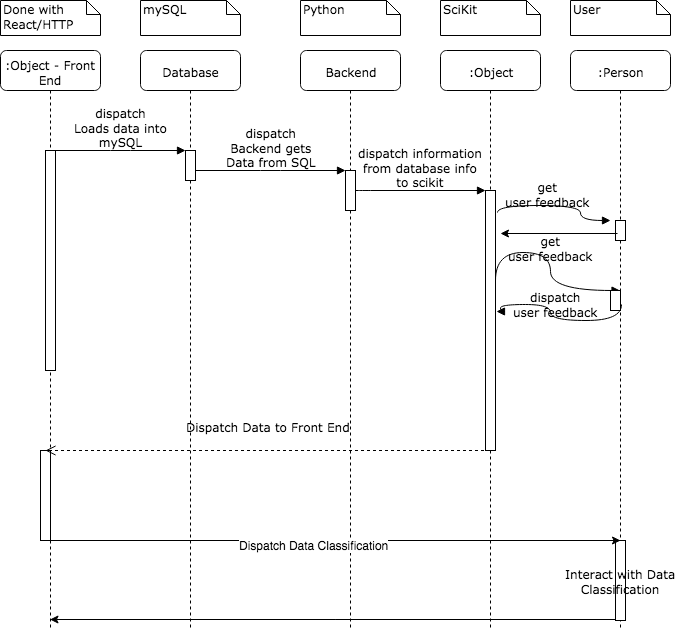
\includegraphics[scale = 0.52]{YarmSequenceDiagram.png}
\begingroup
\captionof{figure}{Sequence Diagram of Data - Matt Yarmolich}
\endgroup

\paragraph{}Figure 4 gives an overview of the classes that will make up the designed system. The main parts of this diagram pertain to the front end, back end, and the machine learning aspect of the project. This diagram will be used to model our architecture of our project and to determine how all the pieces of the system fit together. 
 \paragraph{} All of these components will be designed to be reusable so that they can be strung together and be reused depending on the users use-case. Unfortunately, the languages we have picked do not lend themselves particularly well for object oriented programming (python is a scripted language and react is based on javascript) so we ultimately decided to split these into files.

\section{Test}
Since our solution includes multiple components written in different languages, testing should almost exclusively be written separately for each individual component, with system-wide acceptance testing completed at the end. Described below are testing methods for each component.

\subsection{Login}

\subsection{Data Upload}
\paragraph{} Testing should be performed with all supported data types. Testing should also be performed with unsupported data types to ensure errors are being caught gracefully. Corrupted or improperly-formatted files should be tested as well, since these will also produce errors. This component should also be tested with bulk-uploading, as users may want to upload a large amount of data files at a time.
\paragraph{} Once files have successfully been uploaded, their processed output should be tested for consistency with the source file. Ensure that no values are missing, and the data follows the same structure as the source file.
\paragraph{} Additionally, all other functionality of the Upload Files screen should be functionally tested. Ensure that all buttons work in all states, and users do not get trapped in any states due to unhandled exceptions.

\section{Issues}
[Any issues or open questions should be described here.]

\appendix
\section{Glossary}
Define all the terms necessary to properly interpret the software architecture, including acronyms and abbreviations. You may wish to build a separate glossary that spans multiple projects or the entire organization, and just include terms specific to a single project in each software architecture.

\section{Issues List}
This is a dynamic list of the open architecture issues that remain to be resolved, including TBDs, pending decisions, information that is needed, conflicts awaiting resolution, and the like.
\end{document}
